% !TEX root = main.tex

\documentclass[a4paper, 11pt]{article}
\usepackage[lined]{algorithm2e}
\usepackage{comment} % enables the use of multi-line comments (\ifx \fi) 
\usepackage{lipsum} %This package just generates Lorem Ipsum filler text. 
\usepackage{fullpage} % changes the margin
\usepackage{listings}
\lstset{tabsize=2}

\usepackage{bussproofs}
\usepackage{authblk}
\usepackage{amsmath}
\usepackage{amsfonts}
\usepackage{amssymb}
\usepackage{stmaryrd}
\usepackage{amsthm}
\usepackage{mathtools}
\usepackage{url}
\DeclarePairedDelimiter\ceil{\lceil}{\rceil}
\DeclarePairedDelimiter\floor{\lfloor}{\rfloor}

\usepackage{graphicx}
\graphicspath{ {images/} }

\usepackage{listings}
\usepackage{lscape}
\usepackage{polynom}

\usepackage{etoolbox}
\let\bbordermatrix\bordermatrix
\patchcmd{\bbordermatrix}{8.75}{4.75}{}{}
\patchcmd{\bbordermatrix}{\left(}{\left[}{}{}
\patchcmd{\bbordermatrix}{\right)}{\right]}{}{}

\newtheorem{theorem}{Theorem}
\newtheorem{lemma}{Lemma}
\newtheorem{claim}{Claim}
\newtheorem{definition}{Definition}
\newtheorem{example}{Example}

% Asymptotic Notation
\newcommand{\bigO}[1]{\mathcal{O}(#1)}
\newcommand{\bigOmega}[1]{\Omega(#1)}
\newcommand{\bigTheta}[1]{\Theta(#1)}
\newcommand{\smallO}[1]{o(#1)}
\newcommand{\smallOmega}[1]{\omega(#1)}
\newcommand{\brackett}[1]{\llbracket #1 \rrbracket}
\newcommand{\bracketts}[1]{\llbracket #1 \rrbracket_2}

% Bold
\newcommand{\solution}{\textbf{Solution:}}
\newcommand{\lOp}{\textbf{L}}
\newcommand{\brackets}[1]{\langle{#1}\rangle}
\newcommand{\createSet}[1]{\{#1\}}
\newcommand{\bss}{\backslash}
\newcommand{\lmd}{\lambda}

\author{Jos\'e Abel Castellanos Joo}
\title{On Interpolation and Congruence Closure Algorithms \\ Technical Report}
\affil{Department of Computer Science \\
  University of New Mexico \\
  Albuquerque, NM 87131}
\date{\today}

\begin{document}

\maketitle

\begin{abstract}

  This report presents the activities during \textit{Master Thesis I} given
  by Prof. Deepak Kapur. We discuss algorithms to compute implicational closure,
  congruence closure and interpolants for quantifier-free theories of equality
  over uninterpreted symbols and octagonal formulas. Also, it is discussed the
  implementation of these algorithms, the results and performance obtained.
  Among the objectives of my thesis is the efficient implementation of Prof.
  Kapur's interpolation algorithms and compare performance with \textit{state
    of the art} algorithms for the same theories, mainly using as a reference
  the SAT solver \textit{MathSAT 5}.
  
\end{abstract}

\section{Implicational Closure}

This section discusses the implicational closure algorithm in \cite{DOWLING1984267}.
The author of the previous paper refers to the problem of satisfiability of
propositional Horn Clauses. We use the term `implicational closure'
as the algorithm that solves the satisfiability problem of propositional Horn
Clauses. Later in the paper, we use implicational closure as part of other
algorithms.

It is well known from literature that the Boolean satisfiabity problem (SAT)
for propositional formulas is NP-complete \cite{Cormen:2009:IAT:1614191}.
Nonetheless, if we restrict the class of propositional formulas to Horn Clauses
then it is shown in \cite{DOWLING1984267} the existance of linear algorithm
capable to compute an interpretation for the propositional variables if the
formula is satisfiable, otherwise it halts returning `unsatisfiable formulas'
as a result. For a precise explanation of Horn Clauses, let us provide the
following definitions:

\definition{\cite{Leitsch:1997:RC:260906}} Let $\mathfrak{L}$ be a first-order
language. If $A$ is an \textit{atomic formula} then $A$ and $\neg A$ are
called \textit{literals}. An literal formula $A$ is called \textit{positive
literal} is $A$ is not of the form $\neg B$ for some atomic formula $B$.

\definition{\cite{Leitsch:1997:RC:260906}} A \textit{Horn clause} is a disjunction
of formulas containing a most one positive literal. A \textit{Horn formula} is a
conjunction of Horn clauses.

From the last definition, we can notice two trivial classes of Horn clauses:

\begin{itemize}
\item A does not contain a positive literal: Then $A$ is of the form $\neg P_1
  \lor \dots \lor \neg P_n$ with $n \geq 1$, where each $P_i$ is an atomic formula.
  Equivalently, we can express the above formula as $(P_1 \land \dots \land P_n)
  \rightarrow \bot$ where $bot$ is an unsatisfiable formula (bottom particle).
\item A contains one positive literal: Then $A$ is of the form $Q \lor \neg P_1
  \lor \dots \lor \neg P_n$ with $n \geq 0$, where each $P_i$ is an atomic
  formula. Similarly, we can express $A$ as $(P_1 \land \dots \land P_n)
  \rightarrow Q$.
\end{itemize}

We prefer the second `representation' of Horn clauses due to connections
with logic programming. For convenience, we take standard terminology from
logic programming including $body(H)$ to denote the set of formulae in the
precedent of a Horn clause $H$, and $head(H)$ as the formula in the consequent
of a Horn clause $H$. From this context, a Horn clause with exactly one
positive literal with $n = 0$ is called a `fact', and if $n > 0$ then the
Horn clause is denoted as a `rule'.

The key insight of Gallier's algorithm is precisely the observation mentioned
above about the relation between satisfiability of propositional Horn formulas
and implicational closure. The latter only implies the computation of the
following closure $\mathfrak{C}$:

\begin{itemize}
\item $\text{If } \vdash P \text{ then } P \in \mathfrak{C}$
  
\item $\text{If } P_1 \in \mathfrak{C}, P_2 \in \mathfrak{C}, \dots,
  P_n \in \mathfrak{C} \text{ and } (P_1 \land P_2 \land \dots
  \land P_n) \rightarrow Q \in \mathfrak{C} \text{ then } Q \in \mathfrak{C}$  
\end{itemize}

We notice that the latter closure $\mathfrak{C}$ can be understood as the set
that includes all `facts' of the Horn formula, and successively applies the
`\textit{Modus Ponens}' rules to include new facts from rules if possible.
Gallier's algorithm systematically does this process using a `queue' in order
to avoid unnecessary Modus Ponens calls. Indeed, his algorithm performs this
process partially. For each atomic formula, the author includes
atomic formulae extra variable to keep track of its current truth value.

\begin{itemize}
\item[Step 1.] Initially, all truth values for atomic formulae are set to \texttt{false} 
  and changed only if such atomic formulae are facts in the Horn formula.
\item[Step 2.] Any atomic formula that has changed its truth values from \texttt{false} to
\texttt{true} are pushed into a queue. Two additional data structures keep track
of which Horn clauses include a given atomic formula, and the number of unsatisfied
atomic formulae in the body for each Horn clause. Intuitively, if the number of
unsatisfied formulae in a Horn clause is zero means that the head of the Horn clause
should be included in the closure.
\item[Step 3.] If the queue is empty, then halt and indicate that the Horn formula is
  satisfiable; the truth assignment for each atomic formula is already stored in the
  extended representation mentioned above. Otherwise, pop the first element
  from the queue
  and repeat Step 2.
\end{itemize}

From the previous description of Gallier's algorithm we can see that the
time required is $\bigO{n}$ where $n$ is the number of atomic formulae in the
Horn formula since any atomic formula is never pushed more than once into the
queue.
\section{Congruence Closure}

This problem is a generalization of the previous problem
including first-order formulas (constant and functional symbols)
and equality between terms. Let $TERMS(H)$ be the set of terms in the Horn
formula $H$. Special attention is given to functional symbols, which they
are uninterpreted. Equations are handled using the UNION-FIND
data structure. If there exist In \cite{GALLIER1987233}, the author
introduces to graphs to represent information about the
Horn formula. The first graph is the graph of subterm dependencies
$GT(H)$ in the Horn formula $H$, where all subterms form the vertices of the graph and
a directed edges from node $x$ to $y$ is $y$ is a subformula of
$x$.

\begin{figure}[h]
  \centering
  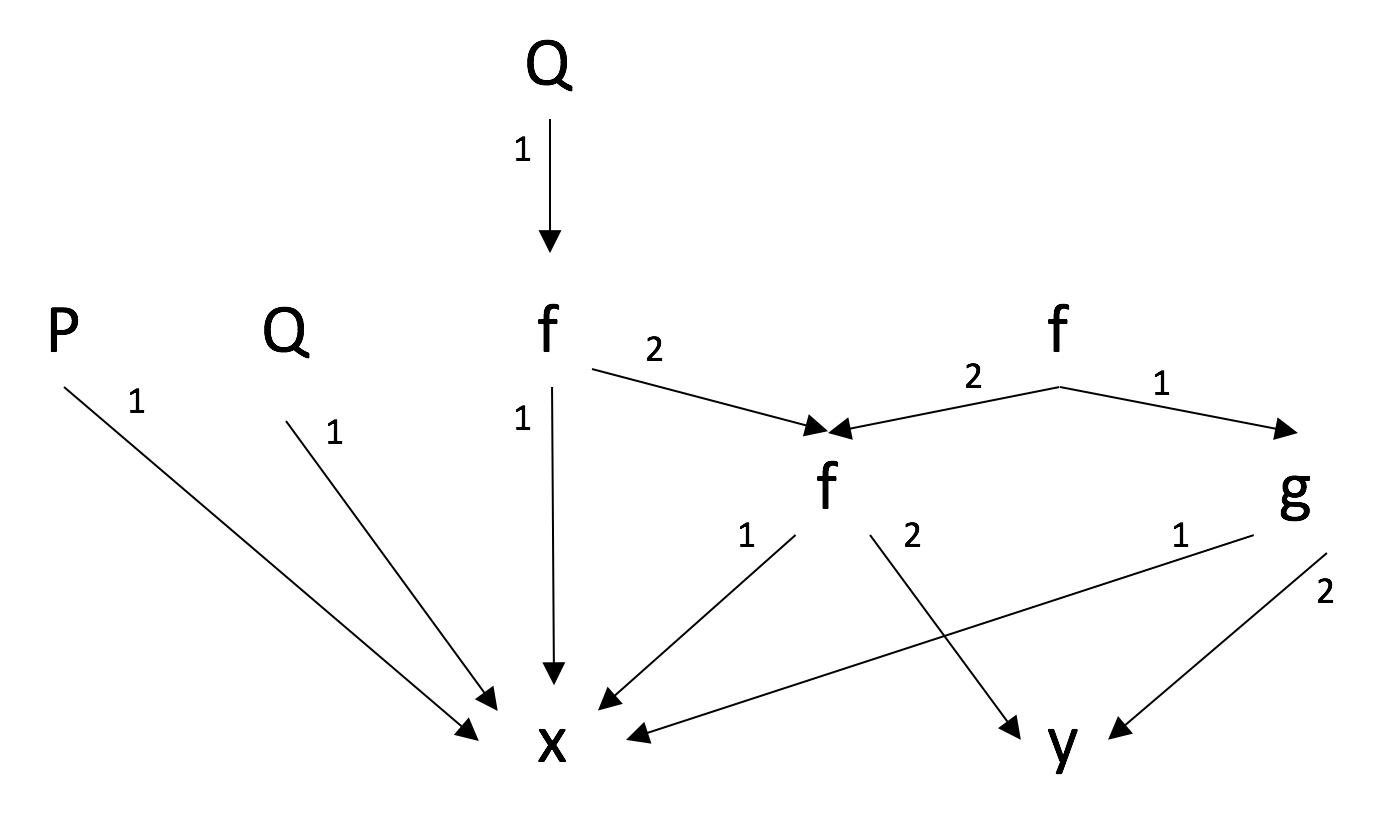
\includegraphics[width=8cm]{GT1}
  \caption{Graph of subterm dependencies for the Horn formula $P(x) :- f(g(x, y), f(x, y)) = y, x = f(x, y) \land Q(f(x, f(x, y))) \land :- Q(x)$}
\end{figure}

The second graph $GC(H)$ encodes the relation between the terms
in the Horn formula $H$, i.e. the vertices are the equations (a predicate $P$
can be `transformed' into an equation of the form $P = \top$)
present in the $H$ (which doesn't include all subterms necessarily), and
there is a directed edge between vertices $x$ and $y$ with label $C$
if there exists a Horn clause $C$ such that $x = head(C)$ and $y \in body(C)$.
The reason for the direction of the edges in $GC(H)$ is because for each node $x$ in
this graph we can check their `successors' with label $C$ (technically the
atomic formulas in the body of the Horn clause $C$) and decide if we should merge
the elements in the equation of $x$ using the UNION-FIND data structure.

\begin{figure}[h]
  \centering
  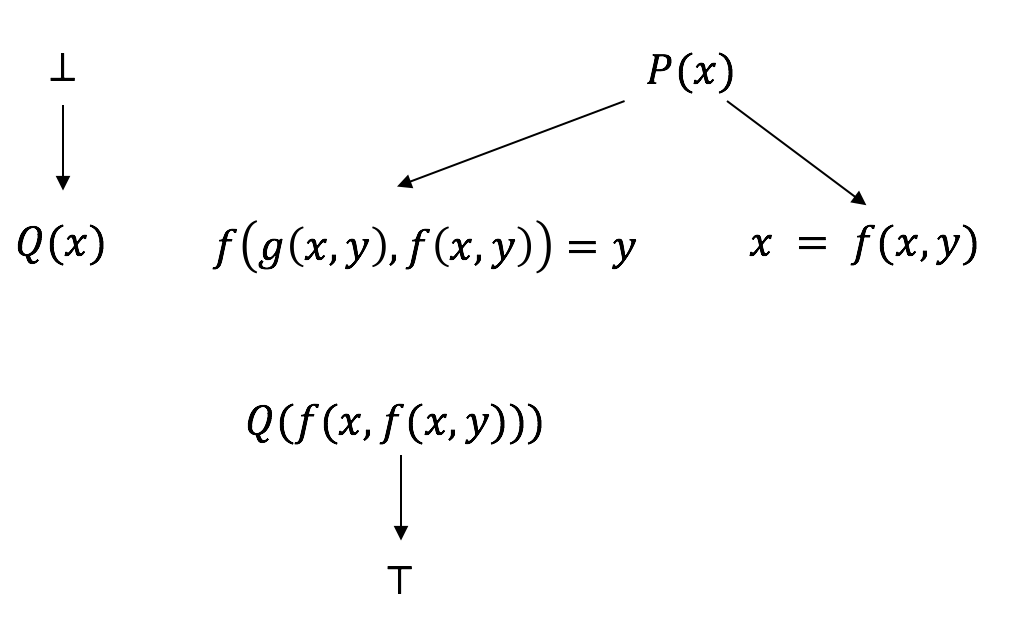
\includegraphics[width=8cm]{GC1}
  \caption{Graph of equations in the Horn formula $P(x) :- f(g(x, y), f(x, y)) = y, x = f(x, y) \land Q(f(x, f(x, y))) \land :- Q(x)$}
\end{figure}

It is important to mention that the author in \cite{GALLIER1987233} generalizes
the concept of equality to describe different types, i.e. we can have more than
one equality between terms. Nonetheless, for the purpose of our work only
one equality is needed between terms. For the latter, some modifications
to the definitions are done in order to keep consistency with our goals.

Also, the author distinguishes two types of closures: in order to compute
the congruence closure of a set of ground Horn clauses implicational and
equational. The implicational closure is essentially the same as described
before in the previous section with the minor change of extending the propositional
formulas to free first-order formulas with equalities. A formal definition of
the equational closure is given as follows:

\definition{\cite{GALLIER1987233}} Let $GT(H)$ be a graph of subterm dependencies for
a given grounded Horn formula $H$ with equalities. An \textit{equational congruence} on $GT(H)$
is a family $R$ of relations $R_i$ (partitions) over $TERMS(H)$ iff:

\begin{itemize}
\item Each $R_i$ is an equivalence relation.
\item For every pair (u, v) in $TERMS(H) \times TERMS(H)$, if the functional names
  of the terms $u, v$ are the same (i.e. they are either both constants or both functions with same name),
  $u \in R_i$, and for each argument of $u$ and $v$ they belong to some relation $R_j$ then $uR_iv$. 
\end{itemize}

The combination of both implicational and equational closure leads to the
congruence closure of a given theory. In fact, the author proved in \cite{GALLIER1987233}
the existance of such closure by interleaving both implicational and equational closure.
Nonetheless, extracting an algorithm from the constructive proof mentioned above
would lead to an inefficient algorithm for computing the congruence closure. Instead, the
author systematically combines a similar approach of implicational closure as we studied
before on the previous section and adding the equational closure component by merging
terms using the UNION-FIND data structure. It is not hard to see that implicational closure
can produce more equations to be merged and the equational closure can lead to new equations
to be satisfiable in the body for Horn clauses. Nonetheless, since there is a finite
number of atomic formulae (equations) and a finite number of Horn clauses, then by interleaving
both closures we can guarantee termination.

The algorithm mentioned in \cite{GALLIER1987233} is an extended version of the algorithm in
\cite{DOWLING1984267} including an \textit{equational congruence} algorithm that checks for
the equational closure mentioned above and the data structure UNION-FIND to deal with equations.
There are two versions of this algorithm. The first one uses a procedure to compute the equational
congruence checking the sucessor for the terms involved each time. As a result, the running time
of the algorithm is $\bigO{m n}$, where $m$ is the number of Horn clauses and $n$ is the number
of atomic formuale. A second refinement utilizes the fast congruence closure algorithm
\cite{Downey:1980:VCS:322217.322228} which obtains a $\bigO{n \log n}$ running time. In order
to become an efficient implementation, several data structures are considered. For each equation
in the Horn formula, we add two records containing the representative element of the left hand side
term and the right hand side term respectively. When merging terms into an equivalence class, it
is considered as the representative the element which has more terms in the tree representation
of the respective equivalence class, hence a `modify the smaller half' heuristic is achieved. This
last heuristic plays an important role to obtain the running time of the algorithm. 

As a side comment, the literature is inconsistent at this point in the sense
that different authors use the same name to describe different problems. In the latter, the term
congruence closure refers to a similar notion of equational closure as studied before in the
previous section.

A `signature' for a functional symbol of the form $f(x_1, \dots, x_n)$ with $n \geq 1$, 
in the sense of \cite{Downey:1980:VCS:322217.322228}, corresponds to the $n-tuple$
$(\alpha(1), \dots, \alpha(n))$, where the function $\alpha : TERMS(H) \rightarrow \mathbb{N}$
is a mapping from the set of terms in the Horn formula to a natural number that encodes
the respective partition in the family of relations $R$. 
The fast congruence closure algorithm described in 
\cite{Downey:1980:VCS:322217.322228} considers two terms to be
`congruent' is their `signatures' are the same. Contrary to the notion of signature in
\cite{GALLIER1987233}, the signtare does no include the name of the respectively terms.
Nonetheless, we can always include functional symbol name as one of the arguments
in the functional symbol signature.

The key addition of the fast congruence closure algorithm is the `Signature Table'. Together
with a UNION-FIND data structure updates only the elements and their signatures as needed,
whereas the previous algorithm updates all terms signatures all the time, even when
they might not be used in the future. Let us describe the operations of these data structures:

UNION-FIND operations:
\begin{itemize}
\item \textit{find(v)}: Given a vertex $v$ in $GT(H)$, return the name of the equivalence
  class containing $v$.
\item \textit{list(e)}: Given a representation $e$ for some equivalence class, return
  the list of vertices with at least one succesor in $e$, i.e. return the set of
  predecessors for all vertices $v$ such that $v \in e$.
\item \textit{union($e_1, e_2$)}: Given two disjoint equivalent classes $e_1, e_2$, combine
  $e_1, e_2$ into a single equivalence class with $e_1$ as representative.
\end{itemize}

SIGNATURE-TABLE operations:
\begin{itemize}
\item \textit{enter(v)}: Given a vertex $v$ from $GT(H)$, store $v$ in the signature
  table with its current signature.
\item \textit{delete(v)}: Given a vertex $v$ from $GT(H)$, delete $v$ from the
  signature table if it is present.
\item \textit{query(v)}: Given a vertex $v$ from $GT(H)$, if there exists a vertex $w$ in
  $GT(H)$ stored in the signature table with same signature as $v$, then return $w$; otherwise
  return $\Lambda$.
\end{itemize}

Two additional sets are needed to keep track of the changes made by the algorithm. The set
\textit{pending} which is a list of vertices to be entered in the signature table, typically
this set is updated when elements are being merged in the UNION-FIND data structure
(equational closure); and \textit{combine}, which is a list of pairs of vertices whose
equivalence classes are to be combined, this structure is updated after performing implicational
closure on the current set of terms and signatures. The fast congruence closure algorithm
is shown in \textbf{Algorithm 1}.

\label{fastCongruenceClosureAlg}
\begin{algorithm}[h]
  $pending = \{v \in V_1 \vert d(v) \geq 1\}$\;
  \While{$pending \neq \empty$}{
    $combine = \emptyset$\;
    \For{each v $\in$ pending}{
      \eIf{$query(v) = \Lambda$}{
        enter(v)\;
      }{
        add (v, query(v)) to combine\;
      }
    }
    $pending = \emptyset$\;
    \For{each (v, w) $\in$ combine}{
      \If{$find(v) \neq find(w)$}{
        \eIf{$|list(find(v))| < |list(find(w))|$}{
          \For{each u $\in$ list(find(v))}{
            delete(u)\;
            add u to pending\;
          }
          union(find(w), find(v))\;
        }{
          \For{each u $\in$ list(find(w))}{
            delete(u)\;
            add u to pending\;
          }
          union(find(v), find(w))
        }
      }
    }
  }
  \caption{The fast congruence closure algorithm}
\end{algorithm}

One invariant of this algorithm is that the signature table
stores vertices in such a way that a signature is never repeated.
This fact comes from observing the for loop at lines 4 - 10. In fact,
any vertex stored at the signature table is the has the most updated
signature and its the reprensetative of the equivalence class.

Regarding implementation details, it is important to mention that the authors
perform a linear transformation on $GT(H)$ such that any functional symbol
contains at most two successors. This is done by a `currying' the formula,
i.e. for any functional symbol $x$ with 1 or 2 successors return the same
vertex representation; otherwise, if the number of successors of $x$ is $n$
with $n > 2$, then introduce a new functional symbol and recursively solve
for the last $n - 1$ arguments of $x$, let us call $x^{'}$ this new functional
symbol, then make an edge between $x$ and its first argument of $x$ and $x^{'}$.

After applying this currying process, all terms will contain at most two
arguments/successors. Because of that, the signature table only requires to
deal with two parts, with the terms with one successor and terms with two
successors. The first part can easily achieve $\bigO{1}$ running time in
all the operations using an array. For the second part, the authors propose
several implementation with different data structures like balanced binary trees,
hash tables, arrays of arrays, etc. Naturally, different running times are
achieved in both running time and space complexity.

To illustrate the algorithm, an example by hand is shown below applying the fast
congruence closure to the equivalence classes $C_0 = \{ \{a, b, f^3 a, f^5 a\}_1 ,\{f a\}_2 ,\{f b\}_3 ,\{f^2 a\}_4 ,\{f^4 a\}_5\}$:

\begin{itemize}
  \item $C_0 = \{ \{a, b, f^3 a, f^5 a\}_1 ,\{f a\}_2 ,\{f b\}_3 ,\{f^2 a\}_4 ,\{f^4 a\}_5\}$
  \item $pending = \{f a, f b, f^2 a, f^3 a, f^4 a, f^5 a\}$
  \item $list(1) = \{f a, f b, f^4 a\}$; $list(2) = \{f^2 a\}$; $list(3) = \{\}$; $list(4) = \{f^3 a\}$; $list(5) = \{f^ 5 a\}$
  \item $combine = \{\}$
  \item $sig\_table = \{(f a, (1))\}$
  \item $combine = \{(f a, f b)\}$
  \item $sig\_table = \{(f a , (1)), (f^2 a , (2) )\}$
  \item $sig\_table = \{(f a , (1)), (f^2 a , (2) ), (f^3 a, (4))\}$
  \item $combine = \{(fa, fb), (fa, f^4 a)\}$
  \item $sig\_table = \{(f a , (1)), (f^2 a , (2) ), (f^3 a, (4)), (f^5 a, (5))\}$
  \item $pending = \{\}$
  \item $C_1 = \{\{a, b, f^3 a, f^5 a\}_1 ,\{f a, f b\}_2  ,\{f^2 a\}_4 ,\{f^4 a\}_5\}$
  \item $sig\_table = \{(f a , (1)), (f^2 a , (2) ), (f^3 a, (4))\}$
  \item $pending = \{f^5 a\}$
  \item $C_2 = \{\{a, b, f^3 a, f^5 a\}_1 ,\{f a, f b, f^4 a\}_2  ,\{f^2 a\}_4 \}$
  \item $list(1) = \{f a, f b, f^4 a\}$; $list(2) = \{f^2 a, f^5 a\}$; $list(3) = \{\}$; $list(4) = \{f^3 a\}$; $list(5) = \{\}$
  \item $combine = \{\}$
  \item $combine = \{(f^2 a, f^5 a)\}$
  \item $pending = \{\}$
  \item $sig\_table = \{(fa, (1)), (f^2 a, (2))\}$
  \item $pending = \{f ^ 3 a\}$
  \item $C_3 = \{\{a, b, f^3 a, f^5 a, f^2 a\}_1 ,\{f a, f b, f^4 a\}_2\}$
  \item $list(1) = \{f a, f b, f^4 a, f^3 a\}$; $list(2) = \{f^2 a, f^5 a\}$; $list(3) = \{\}$; $list(4) = \{\}$; $list(5) = \{\}$
  \item $combine = \{\}$
  \item $combine = \{(f^3 a, f a)\}$
  \item $pending = \{\}$
  \item $sig\_table = \{(fa, (1))\}$
  \item $pending = \{f^2 a, f^5 a\}$
  \item $C_4 = \{\{a, b, f^3 a, f^5 a, f a, f b, f^2 a\, f^4 a\}_1\}$
  \item $combine = \{\}$
  \item $combine = \{(f^2 a, f a)\}$
  \item $combine = \{(f^2 a, f a), (f^5 a, f a)\}$
  \item $pending = \{\}$
  \item $halt$
\end{itemize}
\section{Interpolation Algorithms for quantifier-free EUF and octagonal formulas}

In this section we discuss the novel algorithms by Prof. Kapur. First of all,
we will explain basic notions of interpolants will the goal to understand
the key ideas for Kapur's algorithms.

\definition{} Given formulas $\alpha, \beta$ for some theory $T$ such that
$\vdash \alpha \rightarrow \beta$, then a formula $\gamma$ is called
an \textit{interpolant} of the pair $(\alpha, \beta)$ if
$\vdash \alpha \rightarrow \gamma$, $\vdash \gamma \rightarrow \beta$,
and $\gamma$ contains only common symbols of $\alpha$ and $\beta$. A theory
$T$ is \textit{interpolating} if for all pair of formulas $(\alpha, \beta)$
such that $\vdash \alpha \rightarrow \beta$, and interpolant $\gamma$ of
$(\alpha, \beta)$ can be computed.

In 1957, Craig \cite{craig1957} proved that any theory in first-order logic
is interpolating. An equivalent formulation of the interpolating
property as suggested by Prof. Kapur in one of his talks is that for a
pair $(\alpha, \beta)$ such that $\alpha \land \beta$ is unsatisfiable
(i.e. $\vdash \alpha \rightarrow \neg \beta$),
a formula $\gamma$ is an interpolant of $(\alpha, \beta)$ if
$\vdash \alpha \rightarrow \gamma$ and $\vdash \neg (\gamma \land \beta)$.

From the latter interpolant formula point of view, we can characterize
Prof. Kapur's approach in both of his algorithm as follows. In hindsight, the basic
idea is to perform a collection of `reductions' to the formula $\alpha \land \beta$
until a fixed point is found. Any sequence of these reductions keep the
invariant that for the `current interpolant formula' $\gamma$ with respect
to the pair $(\alpha, \beta)$ it satisfies $\vdash \alpha \rightarrow \gamma$ and
$\vdash \neg(\gamma \land \beta)$, on the other hand the requirement for
$\gamma$ to only contain common symbols of $\alpha, \beta$ is achieved only
when there are no more sequence of reductions to be performed.

Initially, Prof. Kapur's algorithm choose as initial formula the conjunction
$\gamma = \alpha \land \neg\beta$ as the current interpolant formula. This formula satisfies
the invariant proposed above since $\vdash \alpha \rightarrow \alpha$ (tautology),
and $\vdash \alpha \rightarrow \neg\beta$ (by assumption), thus $\vdash \alpha \rightarrow \gamma$.
Similary, we can see that $(\alpha \land \neg \beta \land \beta)$ is unsatisfiable for any $\alpha, \beta$.
Any sequence of reductions satisfy the invariant below because
$\vdash \gamma \rightarrow \gamma^{'}$, where $\gamma^{'}$ is a reduced formula from $\gamma$.
It is worth mentioning that Kapur's algorithm guarantees to remove all uncommon symbols
in the current interpolanting formula. With the latter fact and the invariant
mentioned below we can conclude that the current interpolating formula will
become an interpolant formula of the pairs $(\alpha, \beta)$.

\subsection{Interpolation algorithm for quantifier-free EUF}

This algorithm requires six steps. The first one (preprocessing) performs a flattening process,
which is similar to a well-known algorithm known as the Tseytin transform \cite{Tseitin1983}.
The equations obtained after performing this process are of the form: $f(c_1, \dots, c_k) = d, c = d, c \neq d$,
where $f$ is a functional symbol and each $c_i$, $c$ and $d$ are constants. It is important to mention
that flattening might introduce new symbols, hence in order to distinguish these symbols if they are common
or uncommon symbol Kapur introduced a definition where a new symbol is common if and only all the symbols
in the other term of the equation are common symbols.

The second step generates equivalence classes using the equations obtained in the last step. Using the
UNION-FIND data structure we keep track of the representatives of these classes, prefering common expressions (
expression with only common symbols) as representatives. The last step might require performing
rotations in the three representation, so the UNION-FIND data structure maintains its properties and running
times. For the congruence relation components the algorithm mentioned above is used. The algorithm then replaces
all terms in the set of expressions by their representative in the equivalence class they belong to. If
we obtained equivalence classes with non-common representatives (by construction
the rest of the elements in this class are non-common as well) we can delete it.

The third step involves eliminating uncommon functions symbols. This happens when a functional symbol
$f$ is non-common. Thus, we take all expressions containing the functional symbol $f$ of the form
$f(c_1, \dots, c_k) = c, f(d_1, \dots, d_k) = d$ and we remove them from the set of expression, introducing
the expression $(c_1 = d_1, \dots, c_k = d_k) \rightarrow c = d$. Since this expression is a Horn clause,
many of the algorithms studied before play a crucial role in this algorithm. A forth step exposes uncommon
constants inside functional symbols. Essentially the same process as in step 3 is done.

The fifth step we eliminate uncommon symbols conditionally, i.e. we include the conditions (body of the
Horn clause) needed for a specific equality (head of the respective Horn clause)
to occurs. There are several cases:

\begin{itemize}
\item The body of Horn clause $C$ consists of common expressions and the head of $C$
  contains an uncommon term $u$ on only one side of the equation. We conditionally eliminate
  $u$ in the rest of Horn clauses that contain $u$. We then eliminate $C$ from the current
  interpolant formula since there is no way to eliminate the uncommon expression $u$.
\item The body of Horn clause $C$ consists of common expressions and the head of $C$
  contains only uncommon terms. Then, we can do the same as in the previous case with the
  difference that we replace the equation in the head of the Horn clause $C$ by a symbol $\top$
  which means satisfiable (true). 
\end{itemize}

The last step only states that the obtained current interpolating formula is the interpolant
of the pair $(\alpha, \beta)$.

\subsection{Interpolation algorithm for octagonal formulas}

Contrary to the last interpolantion algorithm, this algorithm uses the
simplification rules:

\begin{equation*}
  \AxiomC{$a x_i + b y_j \leq c$} \AxiomC{$-a x_i + b^{'} y_k \leq d$}
  \AxiomC{$x_i \text{ is an uncommon symbol}$}
  \TrinaryInfC{$b y_j + b^{'} y_k \leq c + d$}
  \DisplayProof
\end{equation*}

\begin{equation*}
  \AxiomC{$a x + a y \leq a c$}
  \UnaryInfC{$x + y \leq c$}
  \DisplayProof
\end{equation*}

Applying these rules as necessary to eliminate uncommon symbols might take at most $\bigO{n^2}$
steps. Additionally, this algorithm terminates since the algorithm remove one uncommon symbol
at a time, and, assuming there is a finite number of uncommon symbols, then the algorithm
terminates. 
\section{Implementation}

Currently we have implemented the interpolant algorithms in Haskell. We have tested
the Haskell implementation with the examples provided in Kapur's paper.

\begin{figure}[h]
  \centering
  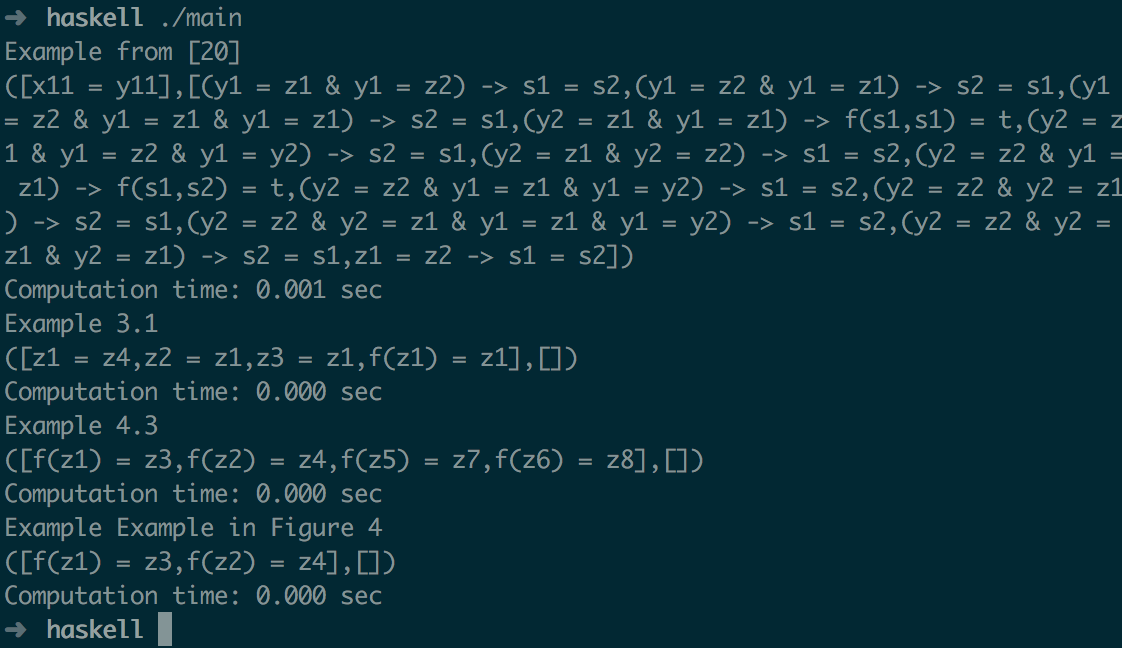
\includegraphics[width=8cm]{eufPerformance}
  \caption{Timming of Haskell program to compute EUF interpolants}
\end{figure}

The implementation of the implicational closure and fast congruence closure
are efficient implementations in C++. We have tested the software with
several automated examples with around 10000 terms. The testing consisted
in checking if the congruence closure was computed as expected, i.e. we checked
every possible pair of terms and check if they are in the congruence
relation iff their successors are already in the congruence relation.

To measure performance we automated several examples. The results of running
time of the algorithm are shown below:

\begin{figure}[h]
  \centering
  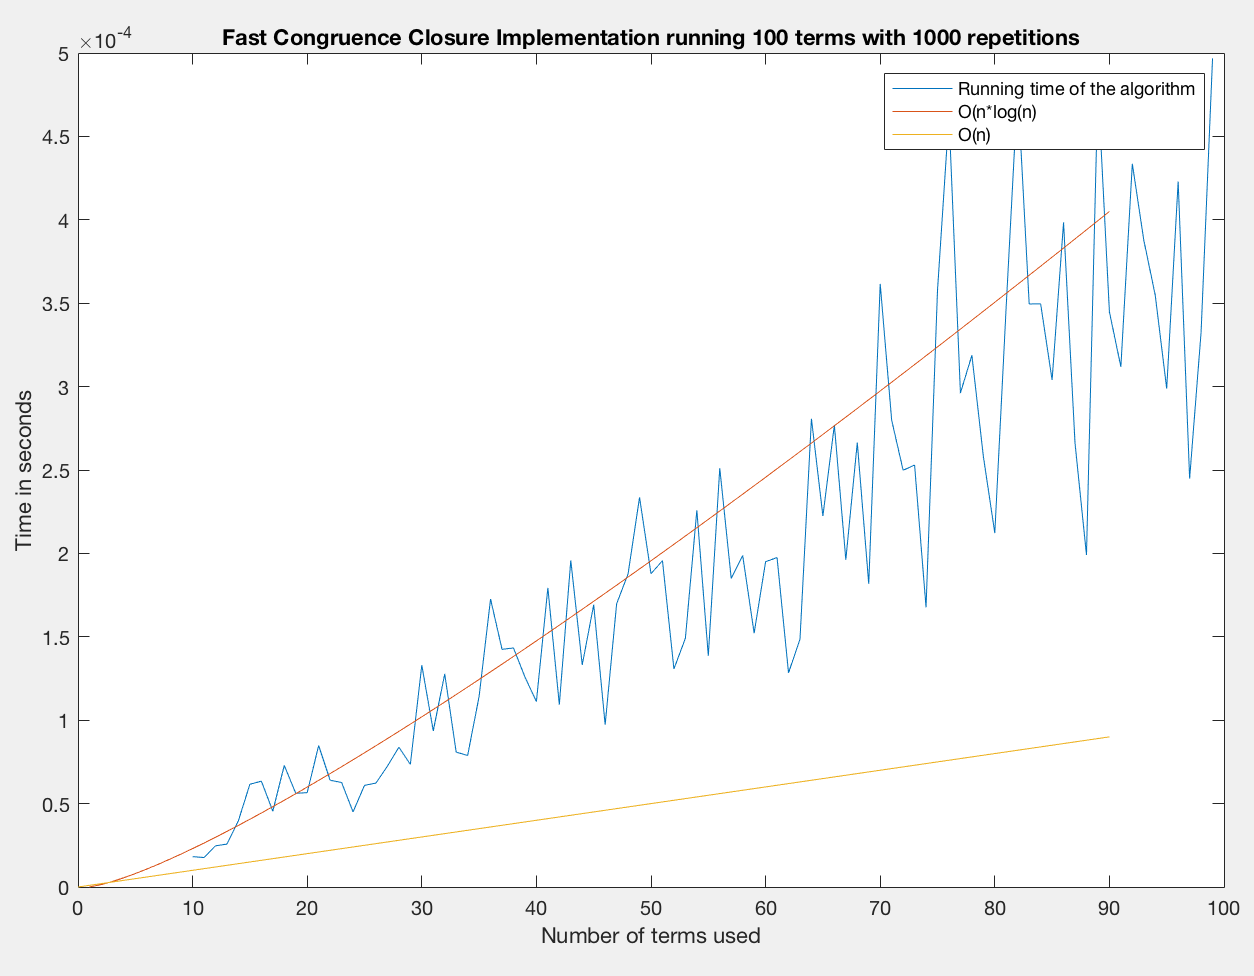
\includegraphics[width=8cm]{100_1000rep}
  \caption{Comparison of running time of the fast congruence closure implementation with
    $\bigO{n \log n}$ and $\bigO{n}$ functions executing 100 terms and doing 1000 repetitions.}
\end{figure}
\begin{figure}[h]
  \centering
  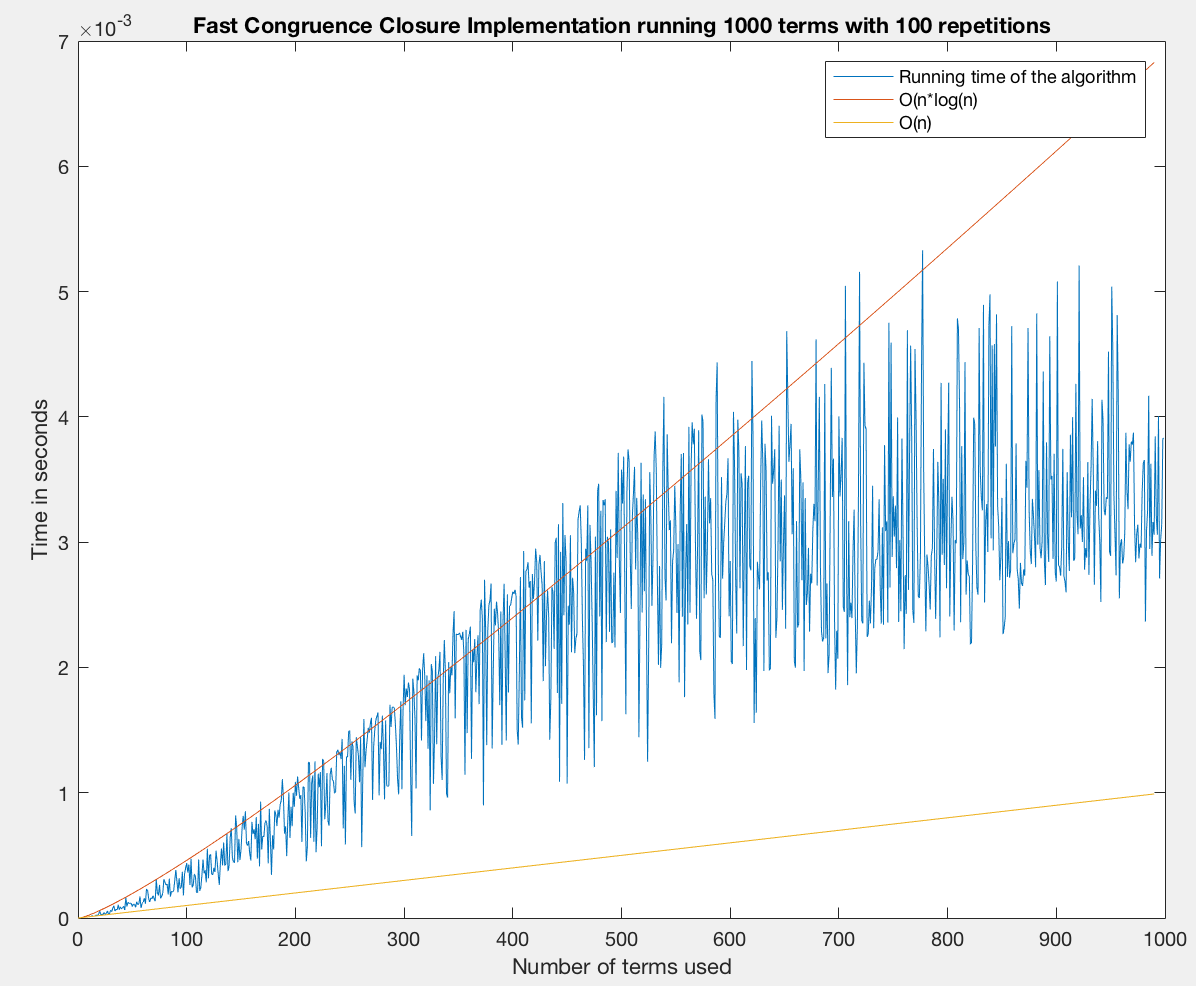
\includegraphics[width=8cm]{1000_100rep}
  \caption{Comparison of running time of the fast congruence closure implementation with
    $\bigO{n \log n}$ and $\bigO{n}$ functions executing 1000 terms and doing 100 repetitions.}
\end{figure}
\begin{figure}[h]
  \centering
  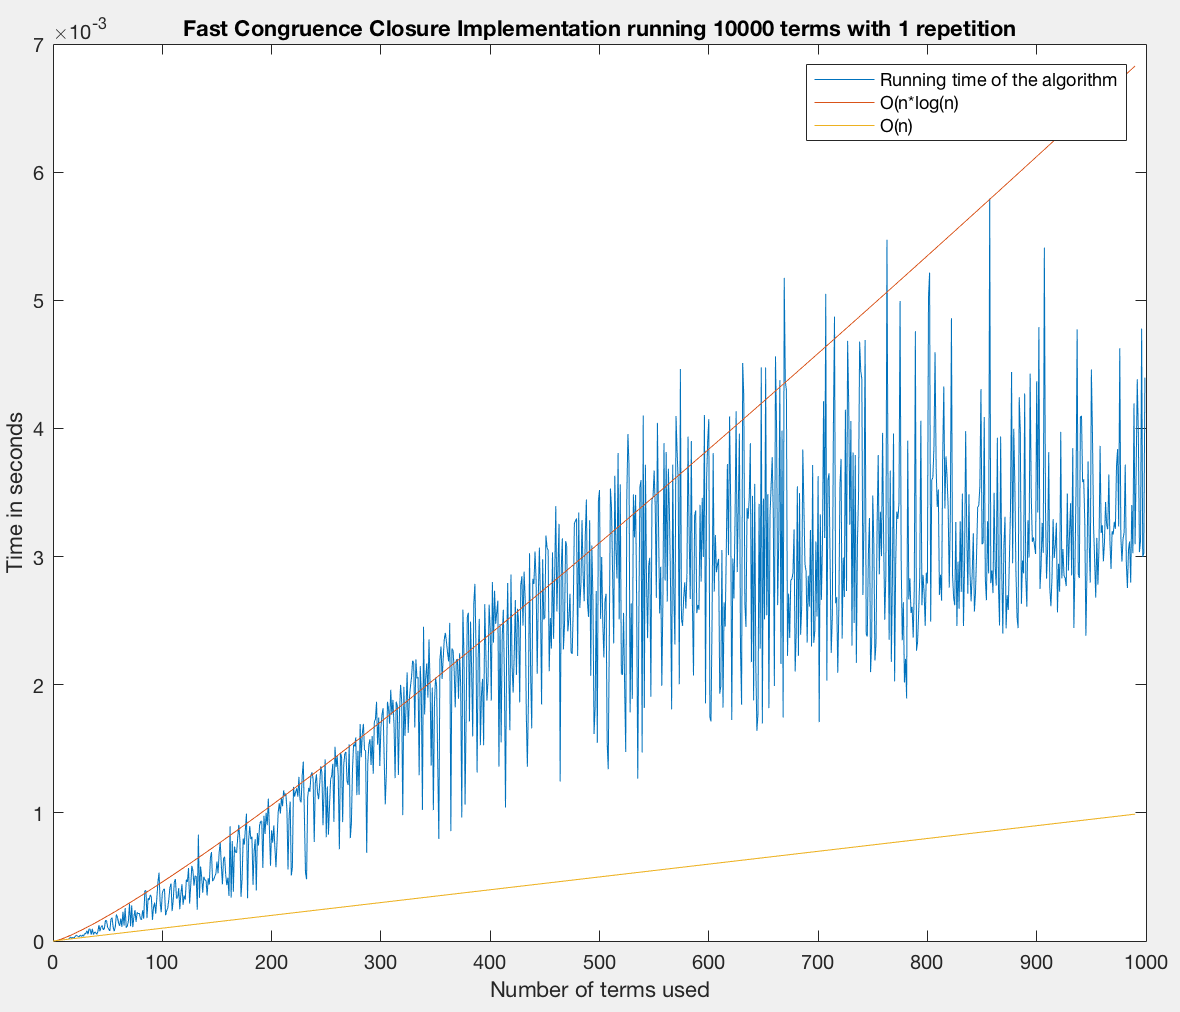
\includegraphics[width=8cm]{10000_1rep}
  \caption{Comparison of running time of the fast congruence closure implementation with
    $\bigO{n \log n}$ and $\bigO{n}$ functions executing 10000 terms and doing 1 repetitions.}
\end{figure}

%\section{Results}
\section{Conclusion}

In this technical report we have discussed several algorithms and their intricate connections.
The exhaustive testing and final performance results indicate the correctness of the
implementation. For the future work, we plan to code the interpolation algorithms
efficiently using C++ and the current fast congruence closure algorithm. The latter
is already defined as a package by itself. Also, it is still pending to compare
the performing results of the current algorithms with the MathSAT 5 package. I predict
that the new interpolantion algorithms should outperform the ones used in the the MathSAT 5
software.


\bibliographystyle{plain}
\bibliography{references}

\end{document}